\documentclass[12pt, a4paper]{article}
\usepackage{geometry}
\geometry{left=2cm}
\geometry{right=1.5cm}
\geometry{top=1cm}
\geometry{bottom=2cm}
\usepackage[T1,T2A]{fontenc}
\usepackage[utf8]{inputenc}
\usepackage[english,russian]{babel}
\usepackage{amsmath}
\usepackage{amsfonts}
\usepackage{amssymb}
\usepackage{makeidx}
\usepackage{mathtext}
\usepackage{graphicx}
\graphicspath{{pictures/}}
\DeclareGraphicsExtensions{.pdf,.png,.jpg,.gif}
\begin{document}
\textit{\textbf{Кластеризация}}  —  процедура, которая собирает данные об объектах и разделяет их на группы (кластеры) по схожим признакам. Используется во многих областях: медицина, археология, маркетинг, \textit{машинное обучение} и др.\\
Нам дано множество точек, необходимо их разбить на группы по какому-либо правилу. Неизвестно, какие использовать правила, расстояния, какое количество кластеров будет в итоге. Это должны решить мы сами и исходя из наших желаний выбрать подходящий алгоритм. Рассмотрим несколько примеров расстояний, которые можно использовать в алгоритме.\\
\begin{itemize}
\itemЕвклидово расстояние: 
\begin{equation}\label{eq:one}
\rho (x, y) = \sqrt{\sum_{i=1}^n (x_i - y_i)^2}
\end{equation}
\itemКосинусное расстояние:
\begin{equation}\label{eq:two}
\rho_{cos} (x, y) = arccos({{\langle X,Y\rangle}\over{\| X \| \| Y \|}})
\end{equation}
\itemМанхеттенское расстояние:
\begin{equation}\label{eq:three}
\rho (x, y) = \sum_{i=1}^n |x_i - y_i|
\end{equation}
\end{itemize}

Все алгоритмы кластеризации делятся на две большие группы: \textit{иерархические} и \textit{плоские}.\\
\textit{Иерархические} алгоритмы разделяются на восходящие и нисходящие. В восходящих предполагается, что каждый элемент, каждая точка изначально — отдельный кластер. В соответствии с введенным расстоянием и оговоренными правилами они объединяются  между собой, образуя всё большие кластеры. В нисходящих наоборот, один большой кластер в процессе алгоритма разделяется на малые. \\
\textit{Плоские} алгоритмы строят одно разбиение объектов на кластеры.

Также кластеры могут быть \textit{пересекающимися} (когда один и более элементов одного кластера одновременно могут принадлежать другим кластерам) и \textit{непересекающимися} (каждый объект принадлежит одному кластеру).
\medskip 
 \medskip 
  \medskip 
   \medskip 
   
\textit{\textbf{Алгоритм k-средних.}}\\Для этого алгоритма необходимо задать необходимое количество кластеров (k) до начала его исполнения. Размещаем на плоскости данные точки и k точек-центроид. Задаём им некоторые цвета или номера, размещаем на плоскости случайно или на своё усмотрение, в зависимости от задачи. Первая итерация алгоритма проверяет для каждой точки её расстояние до каждого из кластеров. Каждая точка помечается цветом кластера, расстояние до которого от неё минимально. Далее вычисляется центр масс каждого кластера, полученного на предыдущем шаге --- суммируем координаты точек по оси абсцисс и делим на количество точек в кластере, это первая координата центроида. Вторая ищется аналогично по оси ординат. После этого происходит перераспределение точек относительно нового положения центров масс, снова меняем цвета каждой точки в цвет того кластера, который находится ближе всего к рассматриваемой точке. Затем вычисляются новые координаты центроид, происходит новое распределение, повторяем этот алгоритм повторяется до момента, пока кластеры не найдут свое «устойчивое» положение, то есть, когда при каждой следующей итерации центры масс не меняют своего положения или меняют, менее чем на на $\epsilon$, который мы задали. Сложность алгоритма по времени, нужному для сходимости, равна $2^{\Omega(\sqrt{n})}.$
\begin{figure}[h!]
\center{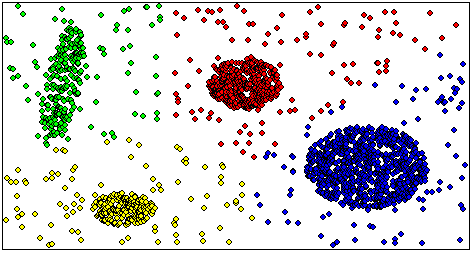
\includegraphics{k-means}}
\caption{Результат работы алгоритма k-средних.}
\label{fig:k}
\end{figure}
\medskip 
 \medskip 
  \medskip 
   \medskip 
   
\textit{\textbf{Алгоритм DBSCAN.}}\\Density-based spatial clustering of applications with noise (плотностной алгоритм пространственной кластеризации с присутствием шума). Алгоритм вычисляет расстояния между всеми точками. До начала работы алгоритма задаем максимальное расстояние, при котором считаем две точки «соседями», то есть, они расположены достаточно близко друг к другу. Также задаём число N -- минимальное количество точек-соседей, чтобы точка считалась в кластере основной, если таких точек меньше N, но не 0, она считается граничной. \\\textit{Немного подробнее о точках:}
\begin{itemize}
\item\textbf{Основная точка.} У точки N и более точек-соседей, которые вместе образуют кластер.
\item\textbf{Граничная точка.} У точки есть «соседи», их меньше N, но хотя бы один из них принадлежит кластеру.
\item\textbf{Шум.} У точки нет «соседей» или их меньше, чем N, но ни один из них не принадлежит ни одному кластеру.
\end{itemize}
После выполнения алгоритма имеем картину с кластерами, их граничными точками и шумом. Время работы: $\mathcal{O}(n*log(n)).$
\begin{figure}[h!]
\center{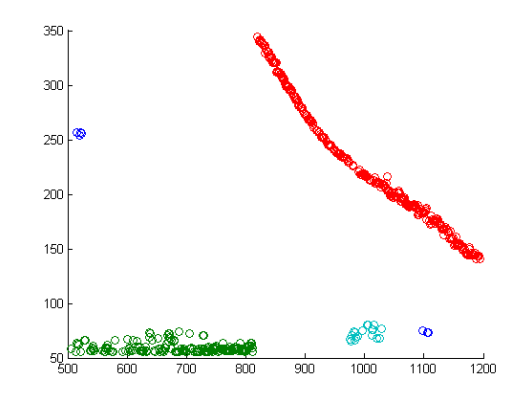
\includegraphics{dbscan}}
\caption{Результат работы алгоритма DBSCAN.}
\label{fig:dbscan}
\end{figure}
\medskip 
 \medskip 
  \medskip 
   \medskip 
   
\textit{\textbf{Иерархический алгоритм.}}

Изначально все точки считаем отдельными кластерами. До начала работы необходимо задать количество кластеров, которое хотим получить после завершения алгоритма, иначе все точки объединятся в один кластер. Далее придумываем признак, по которому будем объединять кластеры. Например, объединяем кластеры, между центрами масс которых минимальное расстояние.
 На каждой итерации происходит объединение кластеров и пересчет центра масс (если использовать предложенный признак) и завершается алгоритм по достижении нужного количества кластеров. Результат можно представить в виде дендрограммы. \\\textbf{Дендрограмма} --- граф без циклов, построенный по матрице мер близости. Она позволяет изобразить взаимные связи между объектами из заданного множества, её рёбра указывают на расстояние между кластерами (это можно наблюдать на Рис. 3). Поэтому оптимальное разбиение точек на кластеры можно увидеть по рёбрам дендрограммы -- если они длинные и их достаточно мало, то можно «отрезать» рёбра -- провести вертикальную линию, по которым отсечем правую часть дендрограммы и увидим оставшиеся кластеры. \\\textit{(Посмотрим на рисунок 3. Проведем вертикальную линию на отметке 10 -- получим два кластера: \{3, 4, 11, 1, 14, 7, 5, 12, 6, 10, 2, 13\} и \{9, 15, 8\}. Если же отсечем по отметке 5 -- получим 3 кластера: \{3, 4, 11, 1, 14, 7, 5, 12, 6, 10, 2, 13\}; \{9, 15\} и \{8\})}
 \begin{figure}[h!]
\center{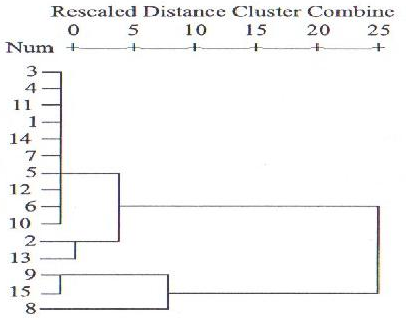
\includegraphics{dendrogr}}
\caption{Результат работы иерархического алгоритма можно представить как дендрограмму.}
\label{fig:dbscan}
\end{figure}
\end{document}